\documentclass[../../docenti.tex]{subfiles}

\begin{document}
\section{Introduzione}

\subsection{Obiettivi}
L'obiettivo di questa unità didattica è quello di consolidare le conoscenze acquisite nel corso di programmazione a blocchi applicandole ad un nuovo ambito, quello della programmazione di microcontrollori.\\
Le logiche di programmazione sono quelle viste in classe, il microcontrollore aggiunge la possibilità di interagire con il mondo esterno attraverso sensori e attuatori, consentendo esercizi e progetti più interattivi e vicini alla vita di tutti i giorni. 

Data la natura di questa unità didattica, non sono previste metodologie di valutazione formativa a fine unità come compiti e quiz. Durante le attività saranno forniti degli spunti per consentire una discussione sul codice e la raccolta di osservazioni informali.

\subsection{Materiali}
Gli esercizi proposti nei capitoli seguenti sono stati pensati per essere svolti da studenti divisi in gruppi di 2-3 persone.

Ogni gruppo necessita di un computer con connessione ad internet. Sarebbe ottimale avere a disposizione un microbit per ogni gruppo, ma è possibile lavorare con il dispositivo simulato presente nell'editor online e mettere a disposizione alcuni dispositivi per test da passare tra gli studenti.

\newpage
\subsection{Micro:Bit}
 MicroBit è un microcontrollore sviluppato da BBC, un'azienda britannica, per insegnare le basi della programmazione e dell'informatica.

\begin{figure}[H]
 	\centering
 	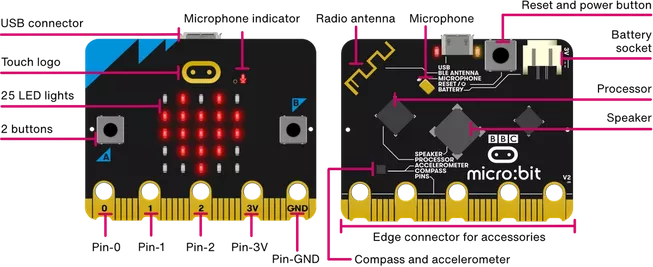
\includegraphics[width=0.8\linewidth]{microbitScheme.png}
 	\caption{Sensori ed attuatori MicroBit versione 1 \parencite{MicrobitOverview}}
 	\label{fig:microbit}
\end{figure}

Il dispositivo è dotato di un display (una griglia di 5x5 LED), due pulsanti e molti sensori\footnote{Una lista completa di sensori e attuatori con esempi di utilizzo è disponibile al seguente indirizzo: \url{https://microbit.org/get-started/user-guide/overview}} tra cui:
\begin{itemize}
	\item accelerometro
	\item bussola
	\item sensore di luminosità
\end{itemize}

\subsection{Make:Code}
MakeCode è un editor online per la programmazione di microcontrollori sviluppato da Microsoft e BBC per MicroBit.\\
L'editor è gratuito e non richiede alcuna installazione, è sufficiente collegarsi al sito \url{https://makecode.microbit.org/} per iniziare a programmare.\\

MakeCode consente di programmare utilizzando programmazione a blocchi oppure utilizzando codice Javascript o Python. In questa unità didattica verrà utilizzata la programmazione a blocchi ma è possibile in qualunque momento converire il codice nelle altre opzioni semplicemente cambiando schermata dell'editor.
\end{document}